\setAuthor{Andreas Valdmann}
\setRound{lõppvoor}
\setYear{2013}
\setNumber{G 9}
\setDifficulty{8}
\setTopic{Dünaamika}

\prob{Jalgpallurid}
Kaks jalgpallurit proovisid trikilööki, kus kaks palli õhus kokku põrkavad.
Jalgpallurid seisid teineteisest $d = \SI{20}{m}$ kaugusel ja andsid samal ajahetkel
sooritatud löögiga kumbki oma pallile algkiiruse $v = \SI{15}{m/s}$. Mis piirkonnas võisid pallid lennul kokku põrgata?
Vastuseks tehke pealtvaates joonis, kuhu on kantud jalgpallurite
asukohad ja kõikvõimalike kokkupõrkepunktide piirkond. Esitage ka selle
piirkonna mõõdud. Võimalike kokkupõrkepunktide kõrgust maapinnast pole
vaja eraldi välja arvutada ega joonisele kanda. Raskuskiirendus
on $g = \SI{9,8}{m/s^2}$. 

\hint
Lihtsuse huvides tasub pallide kiirusi komponentide järgi vaadelda. Vertikaalne komponent $v_z$, horisontaalkomponent pikki jalgpallureid ühendavat sirget $v_y$ ning risti selle sirgega $v_x$. Kokkupõrke hetkel peab risti jalgpallureid ühendava sirgega läbitud vahemaa mõlemal pallil sama olema.

\solu
Vaatame pallide algkiirusi komponentide kaupa. Olgu 1. palli algkiiruse vertikaalkomponent $v_{1\mathrm{vert}}$ ning horisontaalkomponent pikki jalgpallureid ühendavat sirget $v_{1\mathrm{piki}}$ ja risti selle sirgega $v_{1\mathrm{risti}}$. Teise palli jaoks on vastavad komponendid $v\idx{2\mathrm{vert}}$, $v_{2\mathrm{piki}}$ ja $v_{2\mathrm{risti}}$. Kokkupõrke hetkel peavad mõlemad pallid olema läbinud ristsuunas võrdse vahemaa. Kuna pallide ristsuunaline kiirus ei muutu, siis peab kehtima $v_{1\mathrm{risti}}=v_{2\mathrm{risti}}$.\\
Kokkupõrkeks peavad pallid olema jõudnud ka samale kõrgusele. See tingimus on ilmselt täidetud, kui pallide algsed vertikaalkiirused on võrdsed, mille korral on pallid igal ajahetkel samal kõrgusel. Oletame, et pallid võiksid teatud hetkel samale kõrgusele jõuda ka juhul, kui näiteks esimese palli algne vertikaalkiirus on väiksem. Pallide tõusuaeg on arvutatav valemist $t=v_{\mathrm{vert}}/g$. Seega pöördub esimene väiksema vertikaalsuunalise algkiirusega pall varem tagasi. Kui teine pall lõpuks laskuma hakkab, siis liigub esimene pall juba maa poole. Kuna mõlemad pallid kiirenevad võrdselt raskuskiirendusega, siis on laskumisel esimese palli kiirus alati suurem ja teine pall ei jõua selle pallide õhusoleku ajal järele. Seega pole kokkupõrge erinevate vertikaalkiiruste korral võimalik ja peab kehtima $v_{1\mathrm{vert}}=v_{2\mathrm{vert}}$.\\
Kuna algkiirused olid moodulilt võrdsed ja $v^2=v_{\mathrm{vert}}^2+v_{\mathrm{piki}}^2+v_{\mathrm{risti}}^2$, siis peavad ka algkiiruste pikikomponendid olema absoluutväärtuselt võrdsed. Võimalikud kokkupõrkekohad on mõlemast jalgpallurist võrdsel kaugusel ja nende punktihulk moodustab maapinna tasandile projekteerituna sirge, mille otspunktide kaugus mõlemast jalgpallurist on määratud palli maksimaalse lennukaugusega. Selle leidmiseks avaldame näiteks lennuaja, mis on võrdne kahekordse ajaga, mis kulub raskusjõu mõjul vertikaalkiiruse kahanemiseks nullini
\[
t=2\frac{v_{\mathrm{vert}}}{g}.
\]
Selle ajaga liigutakse horisontaalsihis vahemaa
\[
s=v\idx{hor}t=2\frac{v\idx{hor}v\idx{vert}}{g}. 
\]
Suurim lennukaugus saavutatakse, kui $v\idx{vert}=v\idx{hor}=v / \sqrt{2}$ ja seega $s\idx{max}=v^2 / g$.\\
Täisnurksest kolmnurgast leiame kokkupõrkepunktide piirkonna pikkuse
\[
l=2\sqrt{{s\idx{max}}^2-(d/2)^2}=2\sqrt{\frac{v^4}{g^2}-\frac{d^2}{4}},
\]
mille arvväärtus on \SI{41}{m}.

\begin{center}
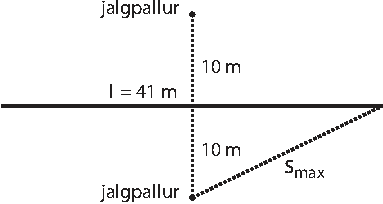
\includegraphics{2013-v3g-09-jalgpallurid}
\end{center}

\probeng{Football players}
Two football players tried a trick move, where two balls would collide in the air. The players stood from each other at a distance $d = \SI{20}{m}$ and hit their balls at the same time, both giving the ball an initial speed of $v = \SI{15}{m/s}$. In what area could the balls collide during the flight? To answer, make a figure from top view where the locations of the players are marked and the area of all the possible collision points. Also give the dimensions of that area. You do not have to find at what height from the ground the possible collision points are. Gravitational acceleration is $g = \SI{9,8}{m/s^2}$.

\hinteng
For simplification the velocities of the balls should be observed as components. The vertical component $v_z$, horizontal component along the line connecting the football players $v_y$ and perpendicular to this line $v_x$. At the moment of the collision the distance covered perpendicularly to the line connecting the footballers must be equal for both balls.

\solueng
Let us observe the initial velocities of the balls by components. Let the vertical component of the first ball’s velocity be $v_{1\mathrm{vert}}$ and the horizontal component along the line connecting the footballers (longitudinal component) $v_{1\mathrm{long}}$ and perpendicular to it $v_{1\mathrm{perp}}$. For the other ball the respective components are $v\idx{2\mathrm{vert}}$, $v_{2\mathrm{long}}$ and $v_{2\mathrm{perp}}$. At the moment of collision both of the balls have to have covered the same distance perpendicularly. Since the perpendicular velocity of the balls does not change then $v_{1\mathrm{perp}}=v_{2\mathrm{perp}}$ must apply.\\
By the moment of collision the balls also have to have reached the same height. This condition is probably fulfilled if the initial vertical velocities of the balls are equal, in which case the balls are at the same height in each moment of time. Let us suppose that the balls would reach the same height in a certain moment of time in the case where the vertical velocity of the first ball is smaller for example. The time it takes the balls to rise is calculated by the formula $t=v_{\mathrm{vert}}/g$. Thus, the first ball with the smaller vertical initial velocity turns back earlier. When the second ball finally starts to descend then the first ball is already moving towards the ground. Because both of the balls accelerate equally under gravitational acceleration then during the descent the velocity of the first ball is always bigger and the second ball does not catch up with that ball during the time in the air. Therefore a collision is impossible with different vertical velocities and $v_{1\mathrm{vert}}=v_{2\mathrm{vert}}$ must apply.\\
Because the initial velocities are equal in module and $v^2=v_{\mathrm{vert}}^2+v_{\mathrm{long}}^2+v_{\mathrm{perp}}^2$ then the longitudinal component of the initial velocities also have to be equal in absolute value. The possible collision locations are at equal distances from both of the footballers and the amount of possible collision points forms a line when projected to a plane. The distance between the ends of the line from each of the footballers is determined by the maximal flight length of a ball. To find this we can express the flight time that is two times smaller than the time it takes the vertical velocity to decrease to zero under gravity force
\[
t=2\frac{v_{\mathrm{vert}}}{g}.
\] 
During this time the following distance is covered horizontally
\[
s=v\idx{hor}t=2\frac{v\idx{hor}v\idx{vert}}{g}. 
\] 
The biggest flight length is achieved when $v\idx{vert}=v\idx{hor}=v / \sqrt{2}$ and therefore $s\idx{max}=v^2 / g$. From a right triangle we find the length of the collision points’ region
\[
l=2\sqrt{{s\idx{max}}^2-(d/2)^2}=2\sqrt{\frac{v^4}{g^2}-\frac{d^2}{4}},
\] 
which has a numerical value 41 m. 
\begin{center}
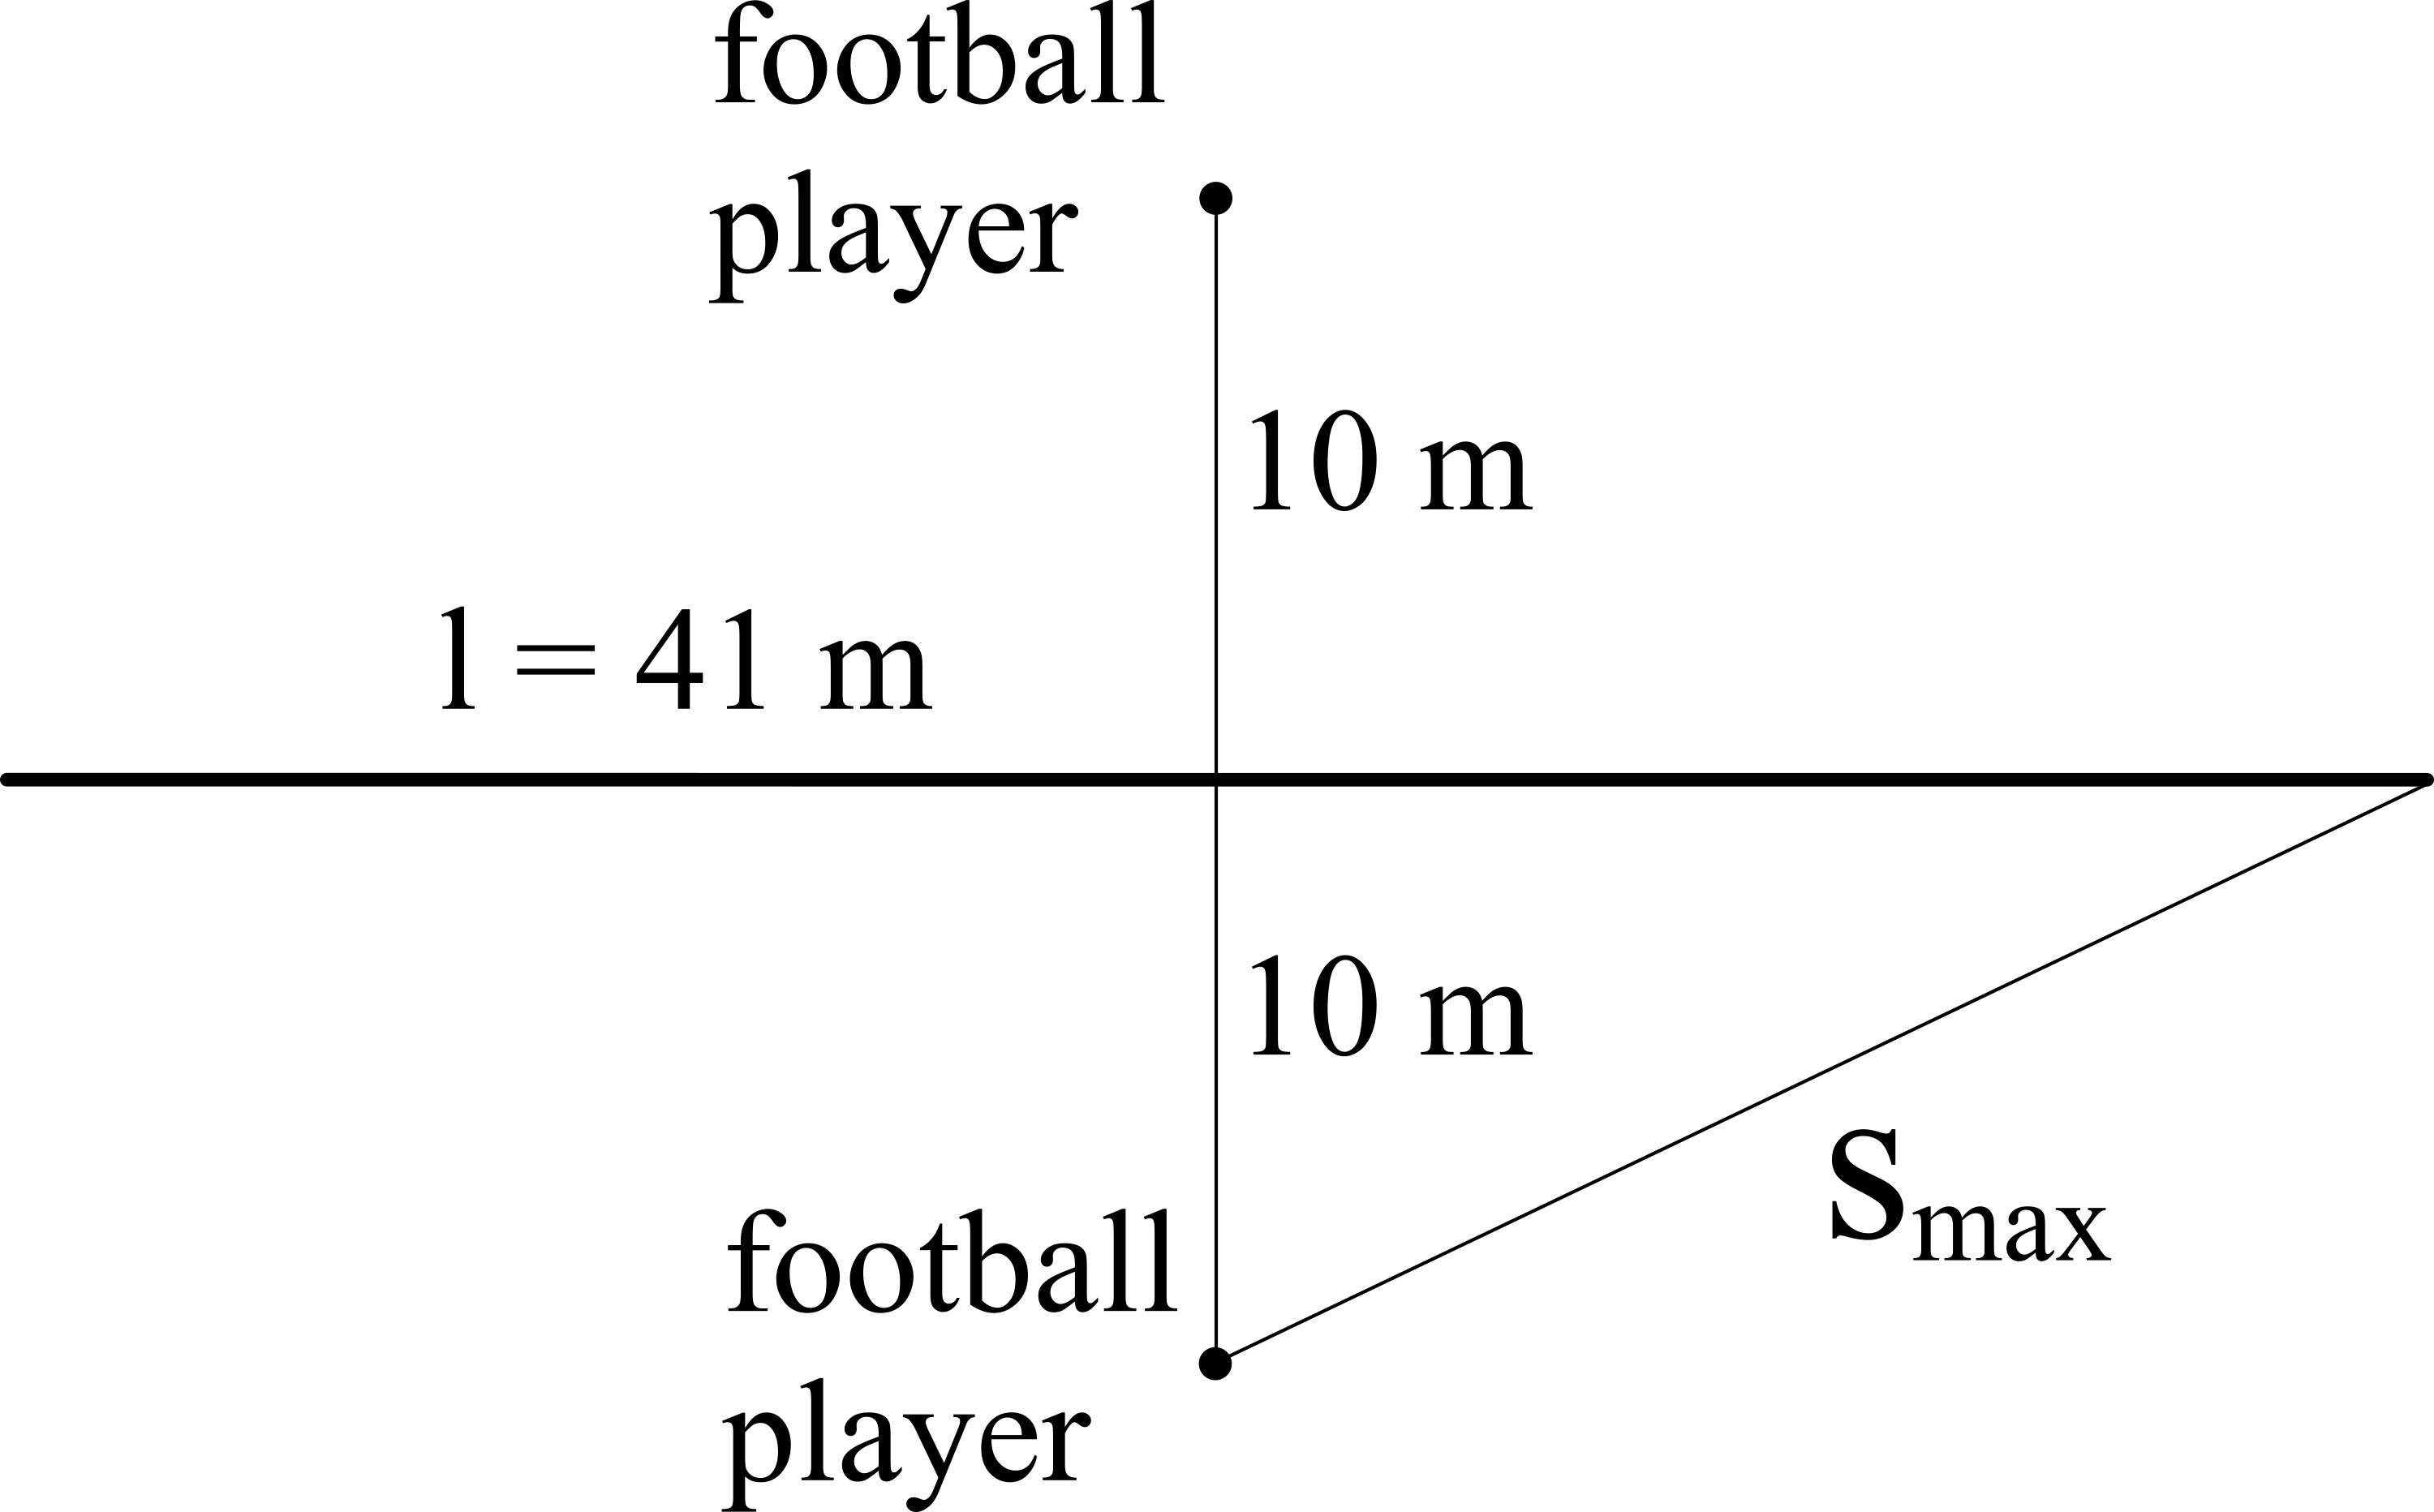
\includegraphics[width=0.5\linewidth]{2013-v3g-09-jalgpallurid_ing}
\end{center}
\probend